\subsection{④}
  \begin{figure}[H]
    \begin{tabular}{ccc}
      \begin{minipage}{.5\textwidth}
        \centering
        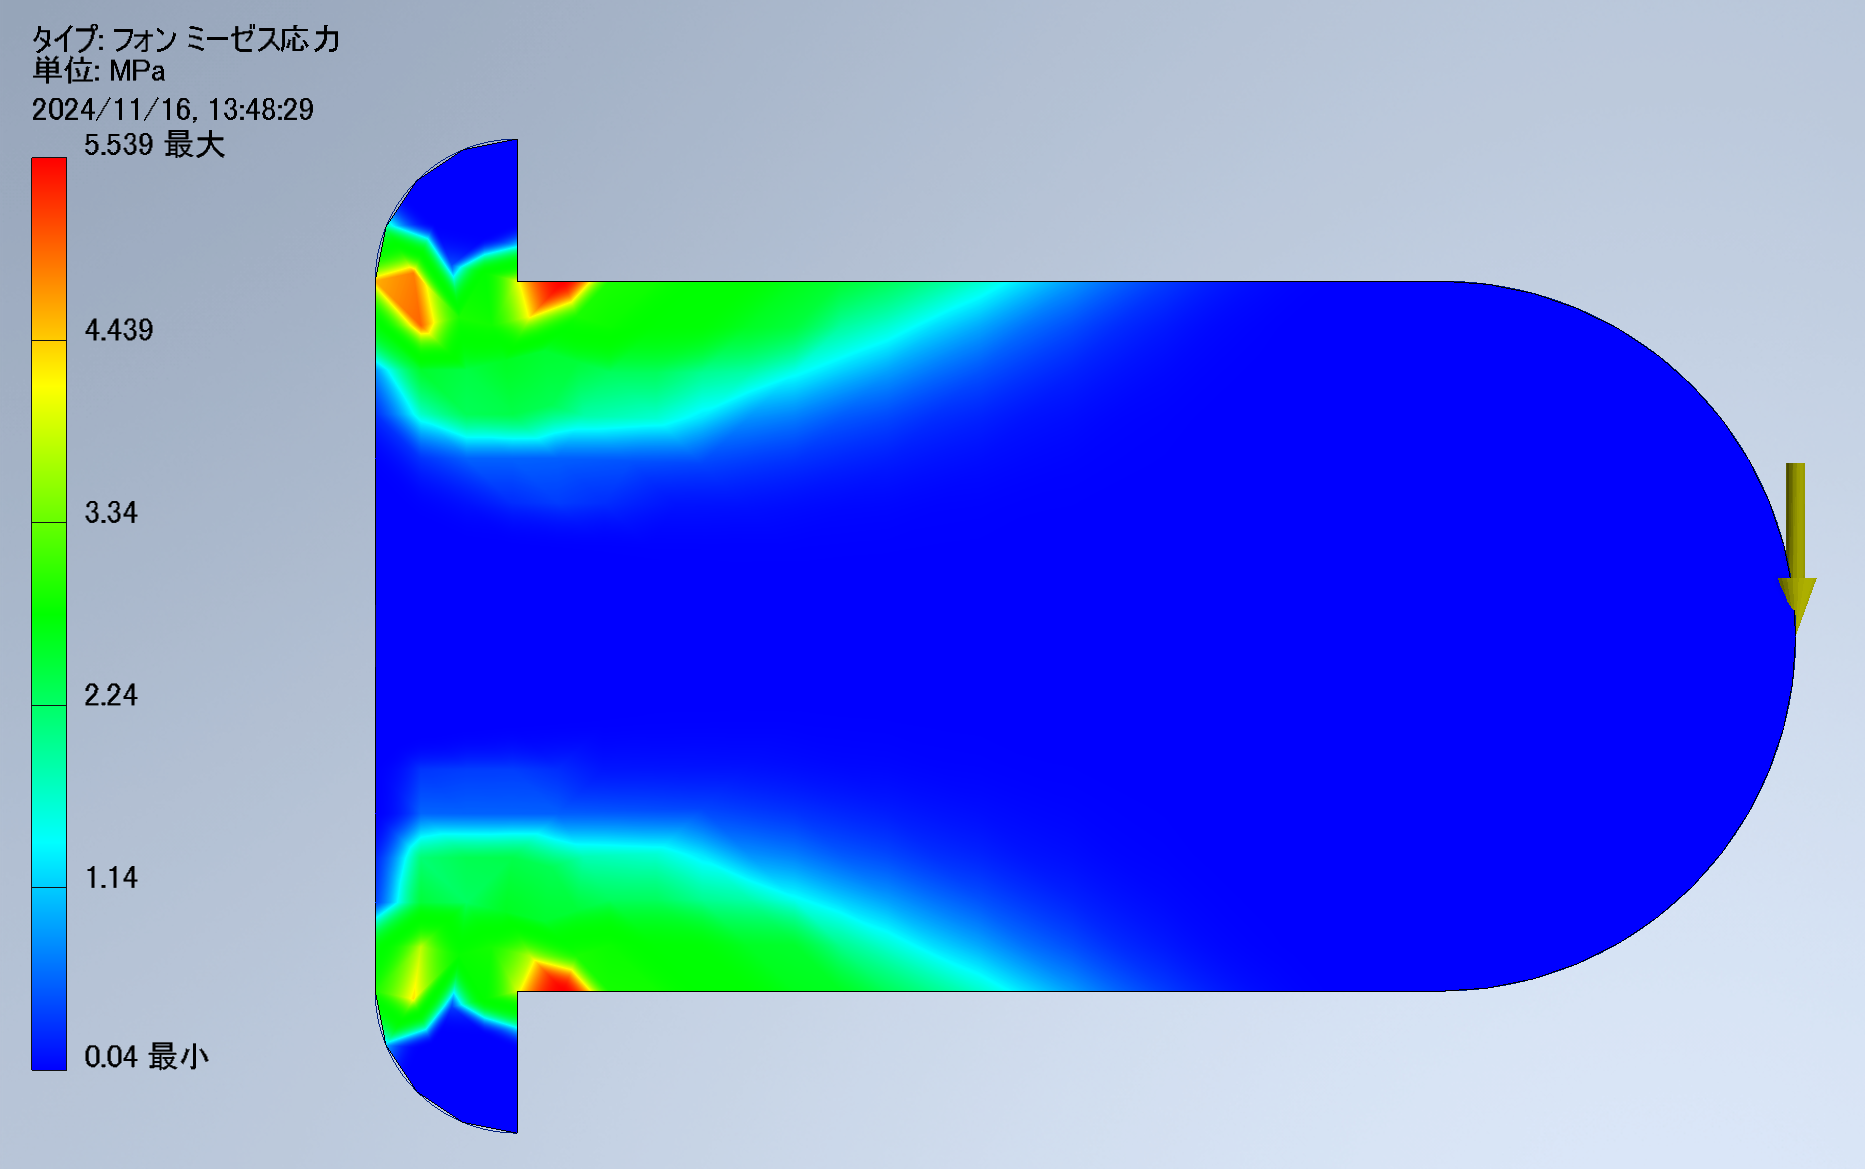
\includegraphics[width=0.99\linewidth]{images/4_voms.png}
        \caption{応力}
        \label{img:4_voms}
      \end{minipage}
      \begin{minipage}{.5\textwidth}
        \centering
        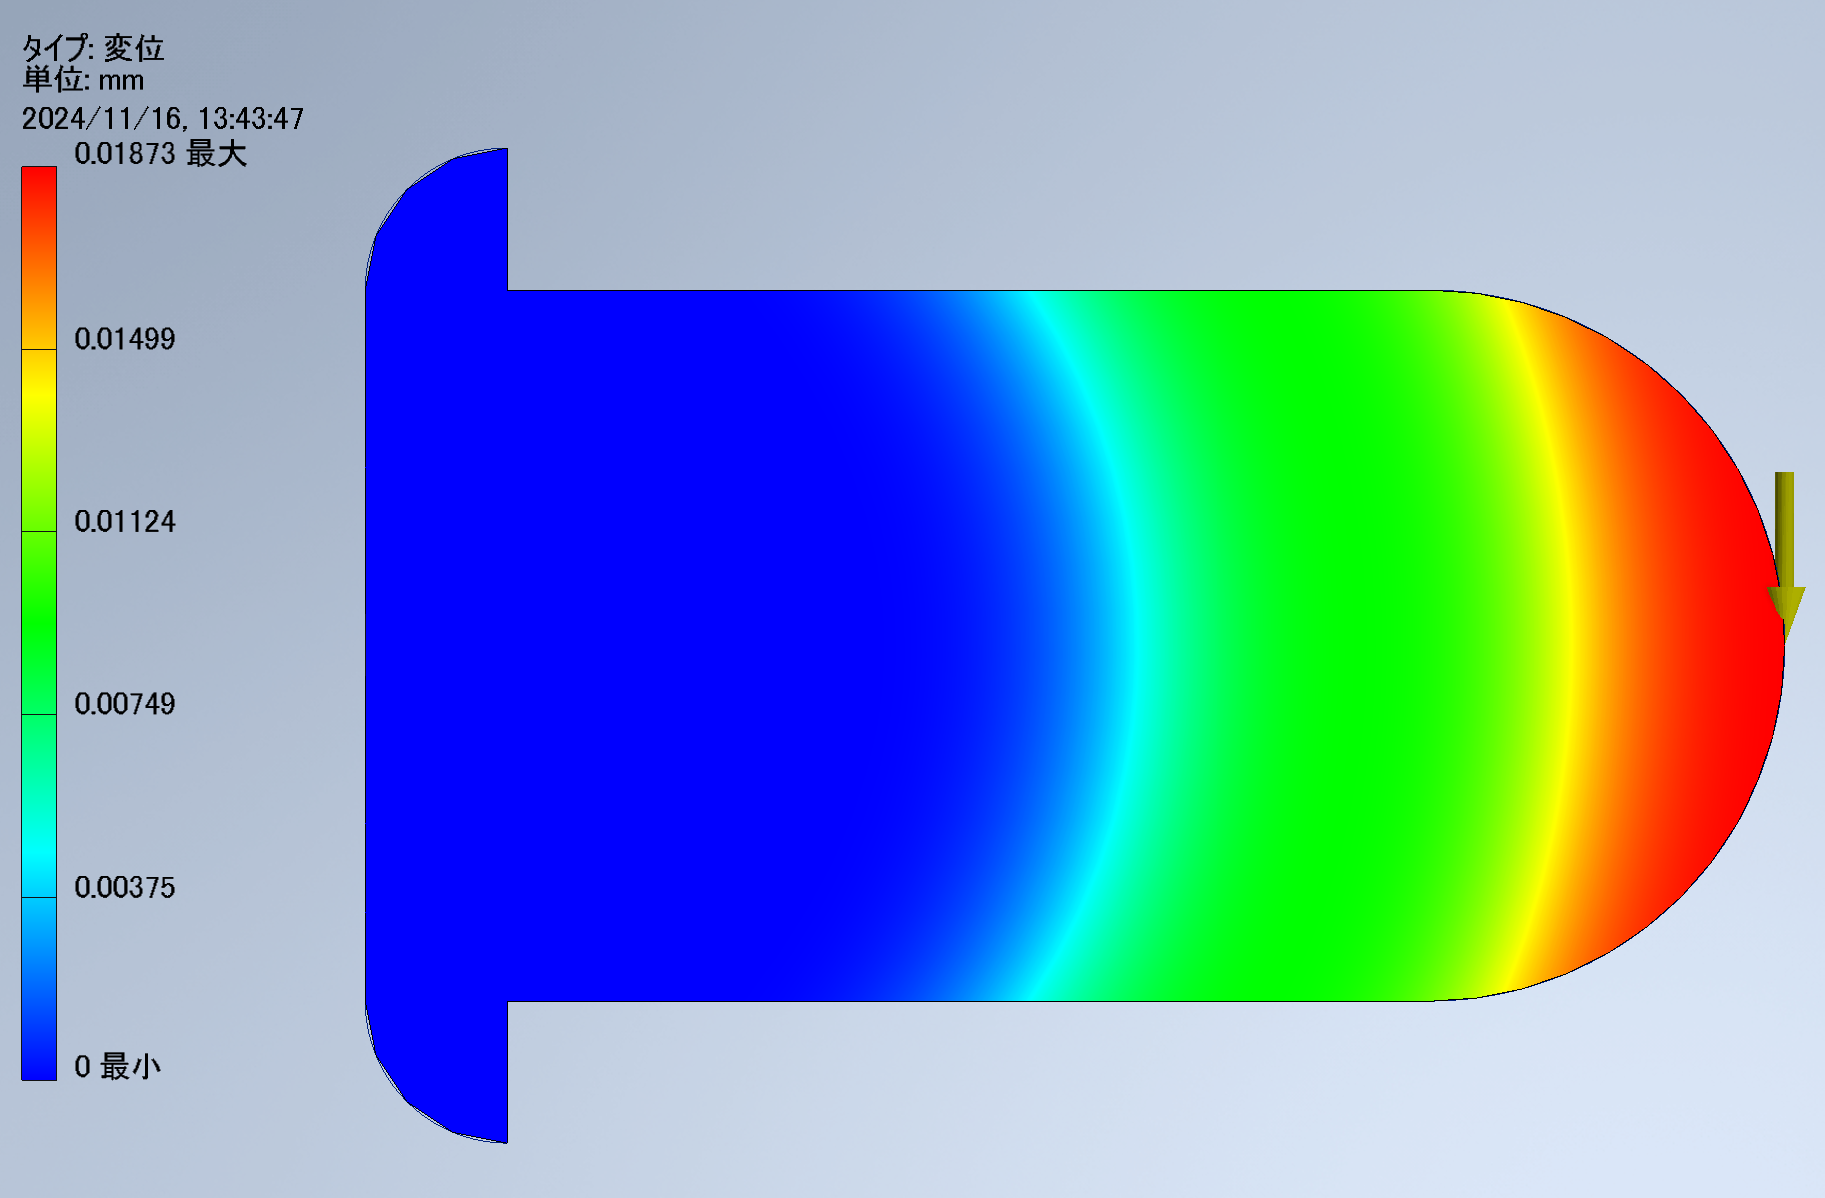
\includegraphics[width=0.99\linewidth]{images/4_disp.png}
        \caption{変位}
        \label{img:4_disp}
      \end{minipage}
    \end{tabular}
  \end{figure}

  ③の解析条件より,補強に充てられる体積は以下.
  \begin{align*}
    V &= 50000 - 47096[mm^3] \\
      &= 2904[mm^3]
  \end{align*}

  
  図\ref{img:3_voms}より応力が大きくかかっている,
  接地面の上下の角を,余裕を持ってそれぞれ体積$1000[mm^3]$の四角柱で補強する.
  このときの$zx$平面の面積は$1000 \div 2.485 \approx 400[mm^3]$.
  補強のパーツの面積は$20 \times 20 [mm^3]$にした.
  接地面が増加しないように接地面の角に,
  半径$20[mm]$のフィレットを施した.このときの解析条件は以下.
  \begin{equation*}
    V \approx 48659[mm^3]
  \end{equation*}

  以上の図より結果としては,変位の最大値は$0.005[mm]$ほど小さくなったが,
  応力の最大値は変化しなかった.そこで,補強のパーツを以下のサイズにして再度実験を行った.
  ($V$ : 梁の体積)
  \begin{itemize}
    \item $50\times8[mm^3]$,$V \approx 49018[mm^3]$
    \item $100\times4[mm^3]$,$V \approx 49069[mm^3]$
    \item $120\times3.3[mm^3]$,$V \approx 49055[mm^3]$
    \item $150\times2.6[mm^3]$,$V \approx 49029[mm^3]$
  \end{itemize}

  \begin{figure}[H]
    \begin{tabular}{ccc}
      \begin{minipage}{.25\textwidth}
        \centering
        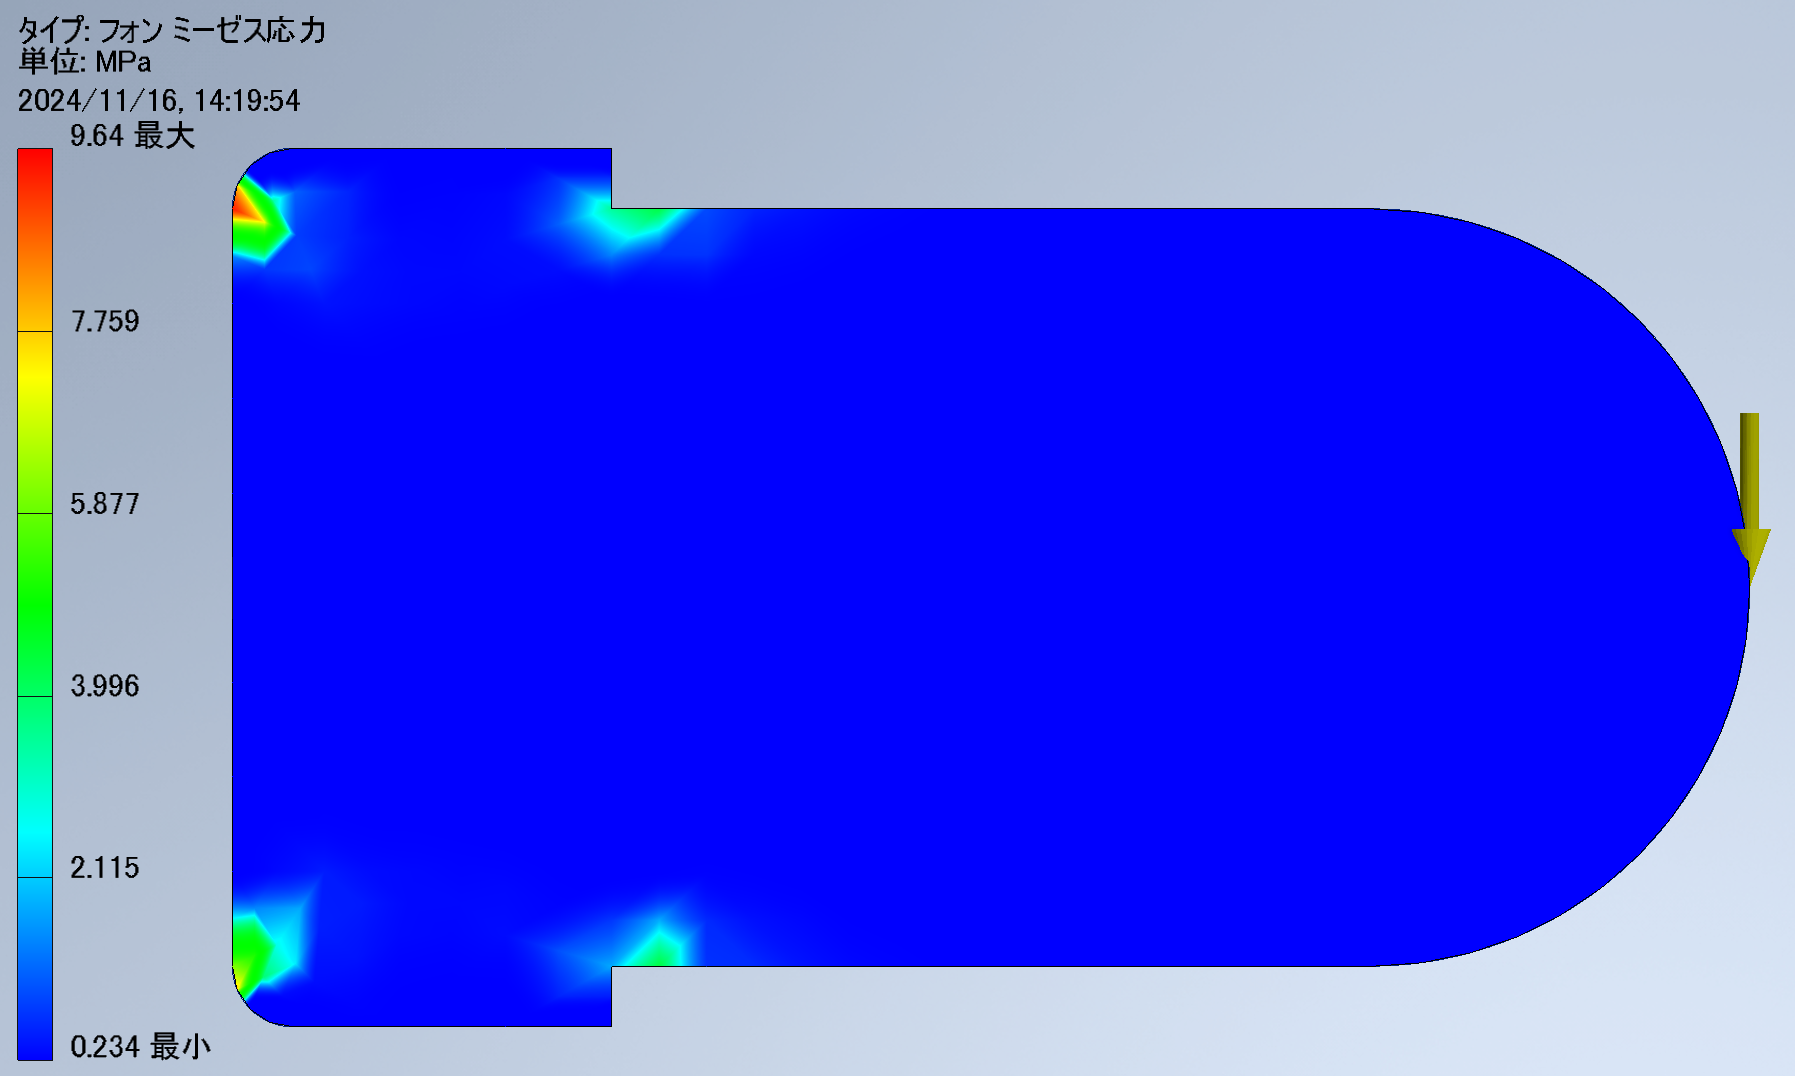
\includegraphics[width=0.99\linewidth]{images/4-3_voms.png}
        \caption{$50\times8[mm^3]$}
        \label{img:4-3_voms}
      \end{minipage}
      \begin{minipage}{.25\textwidth}
        \centering
        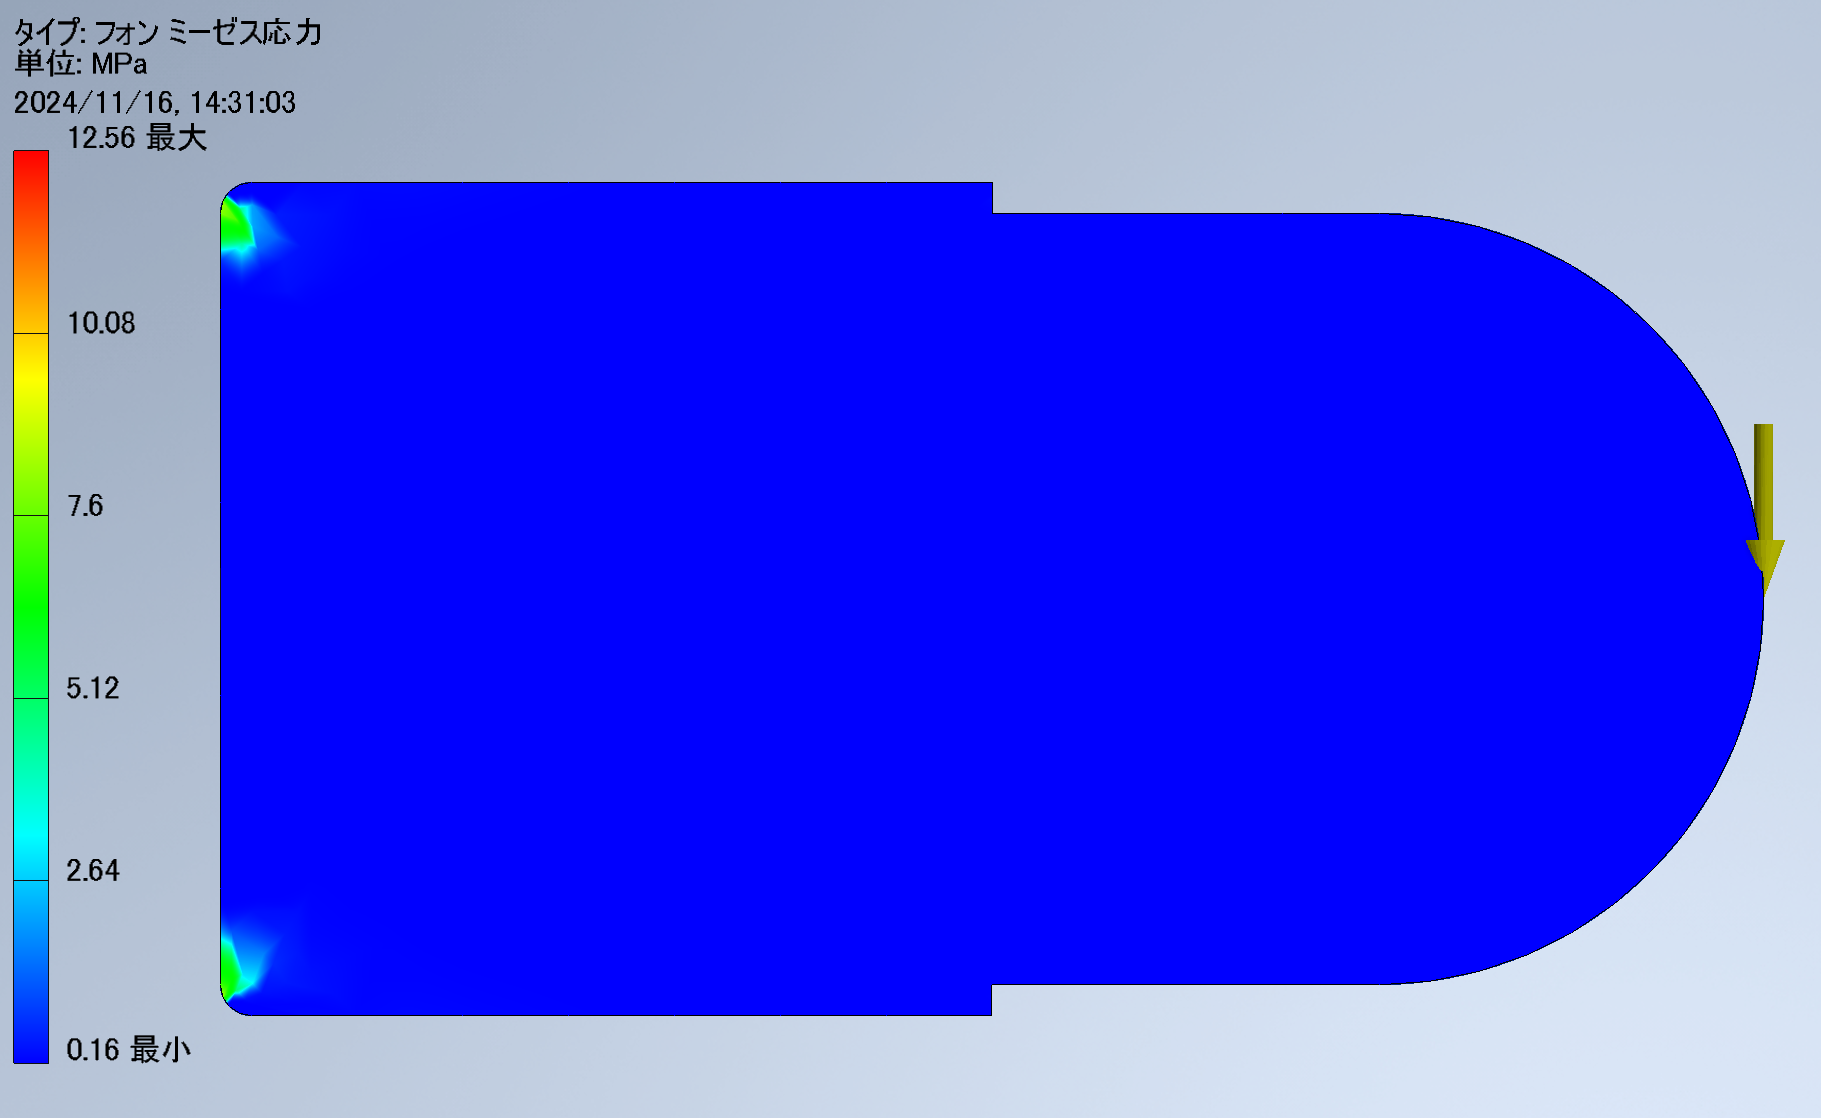
\includegraphics[width=0.99\linewidth]{images/4-6_voms.png}
        \caption{$100\times4[mm^3]$}
        \label{img:4-7_voms}
      \end{minipage}
      \begin{minipage}{.25\textwidth}
        \centering
        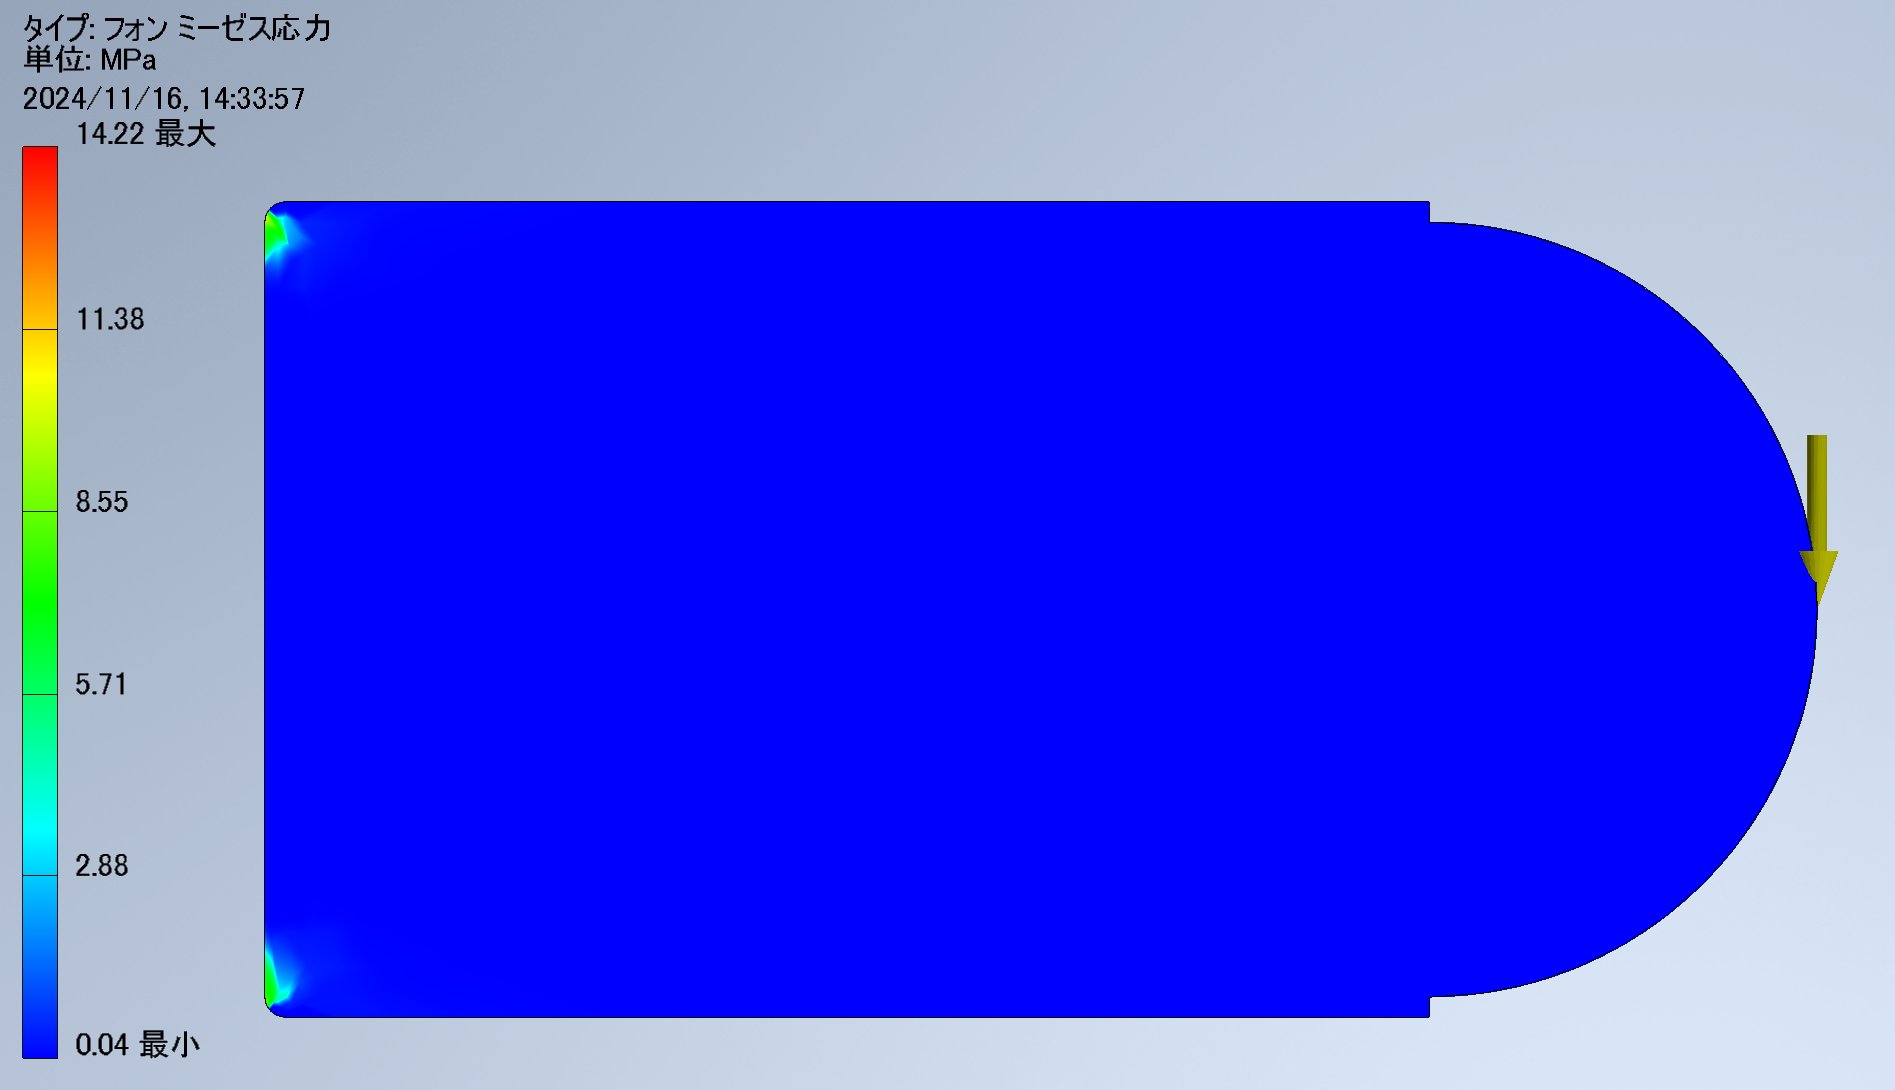
\includegraphics[width=0.99\linewidth]{images/4-7_voms.png}
        \caption{$120\times3.3[mm^3]$}
        \label{img:4-7_voms}
      \end{minipage}
      \begin{minipage}{.25\textwidth}
        \centering
        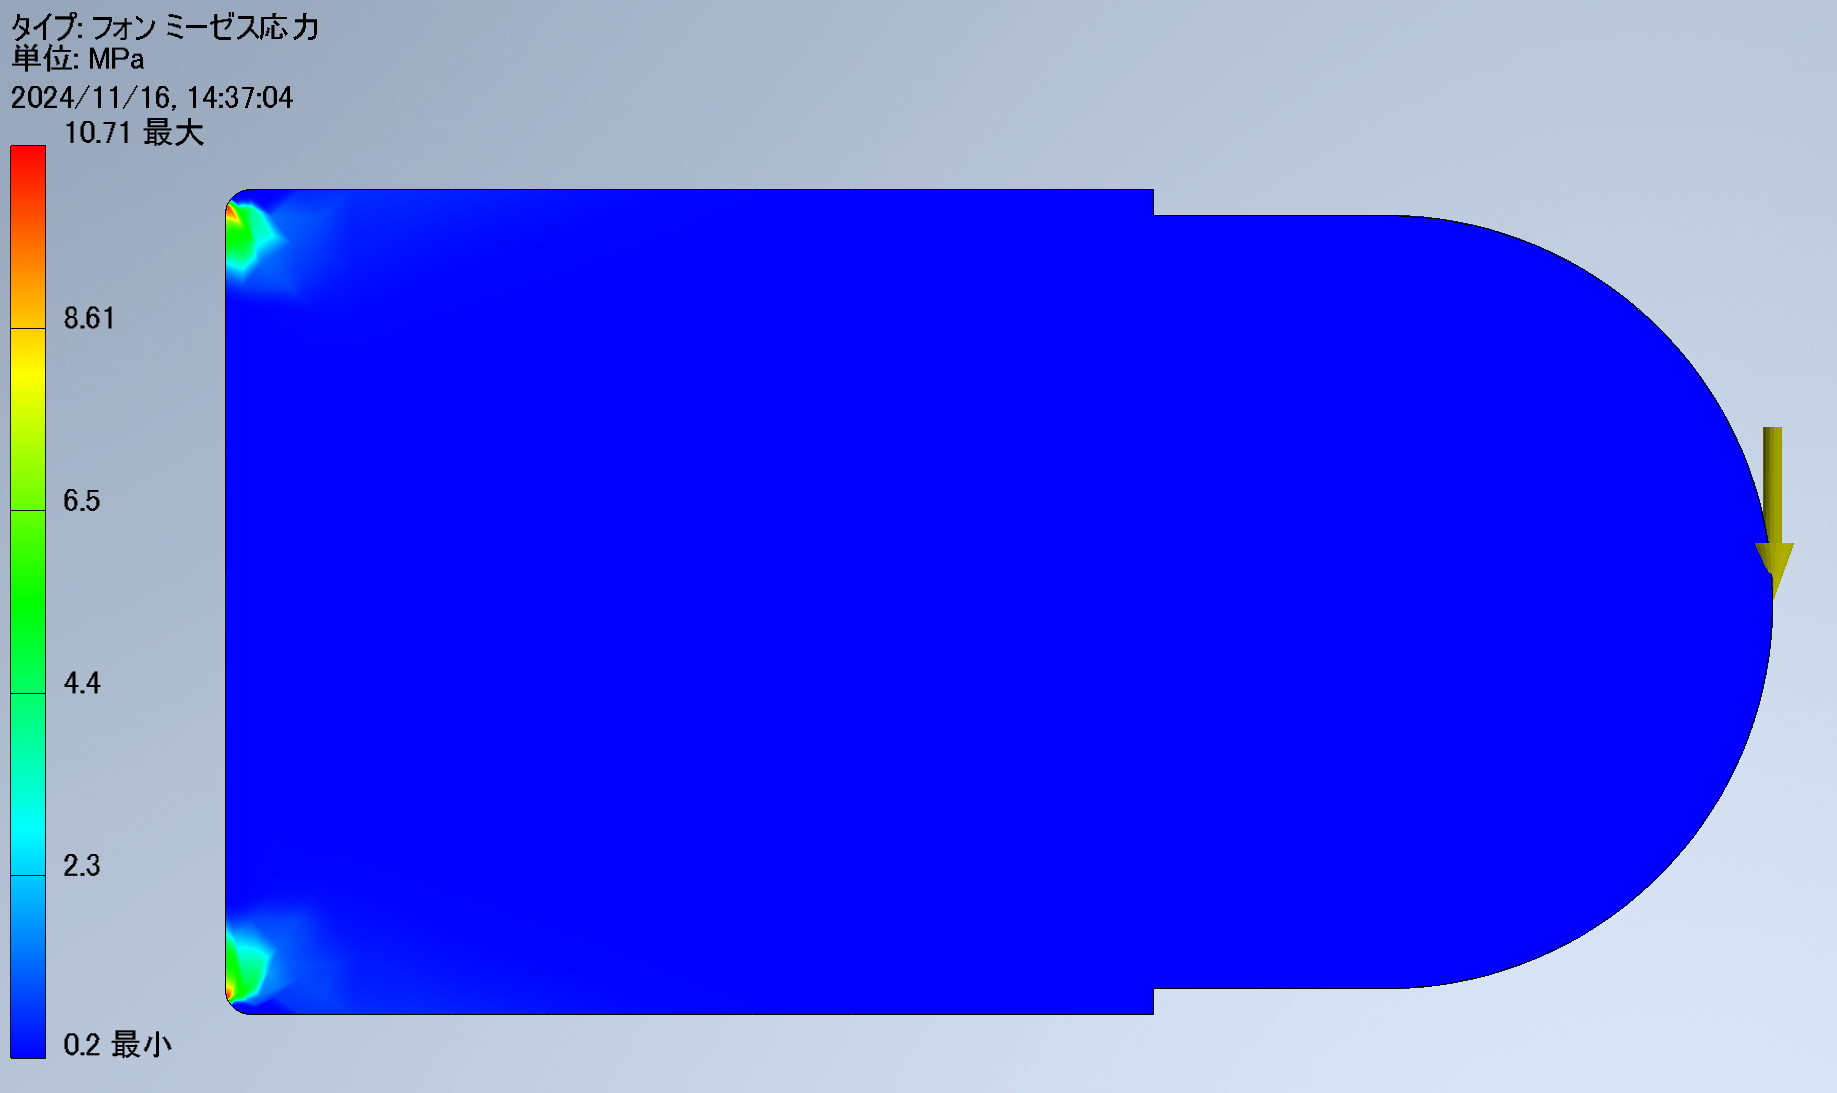
\includegraphics[width=0.99\linewidth]{images/4-8_voms.png}
        \caption{$150\times2.6[mm^3]$}
        \label{img:4-8_voms}
      \end{minipage}
    \end{tabular}
  \end{figure}

  \begin{figure}[H]
    \begin{tabular}{ccc}
      \begin{minipage}{.25\textwidth}
        \centering
        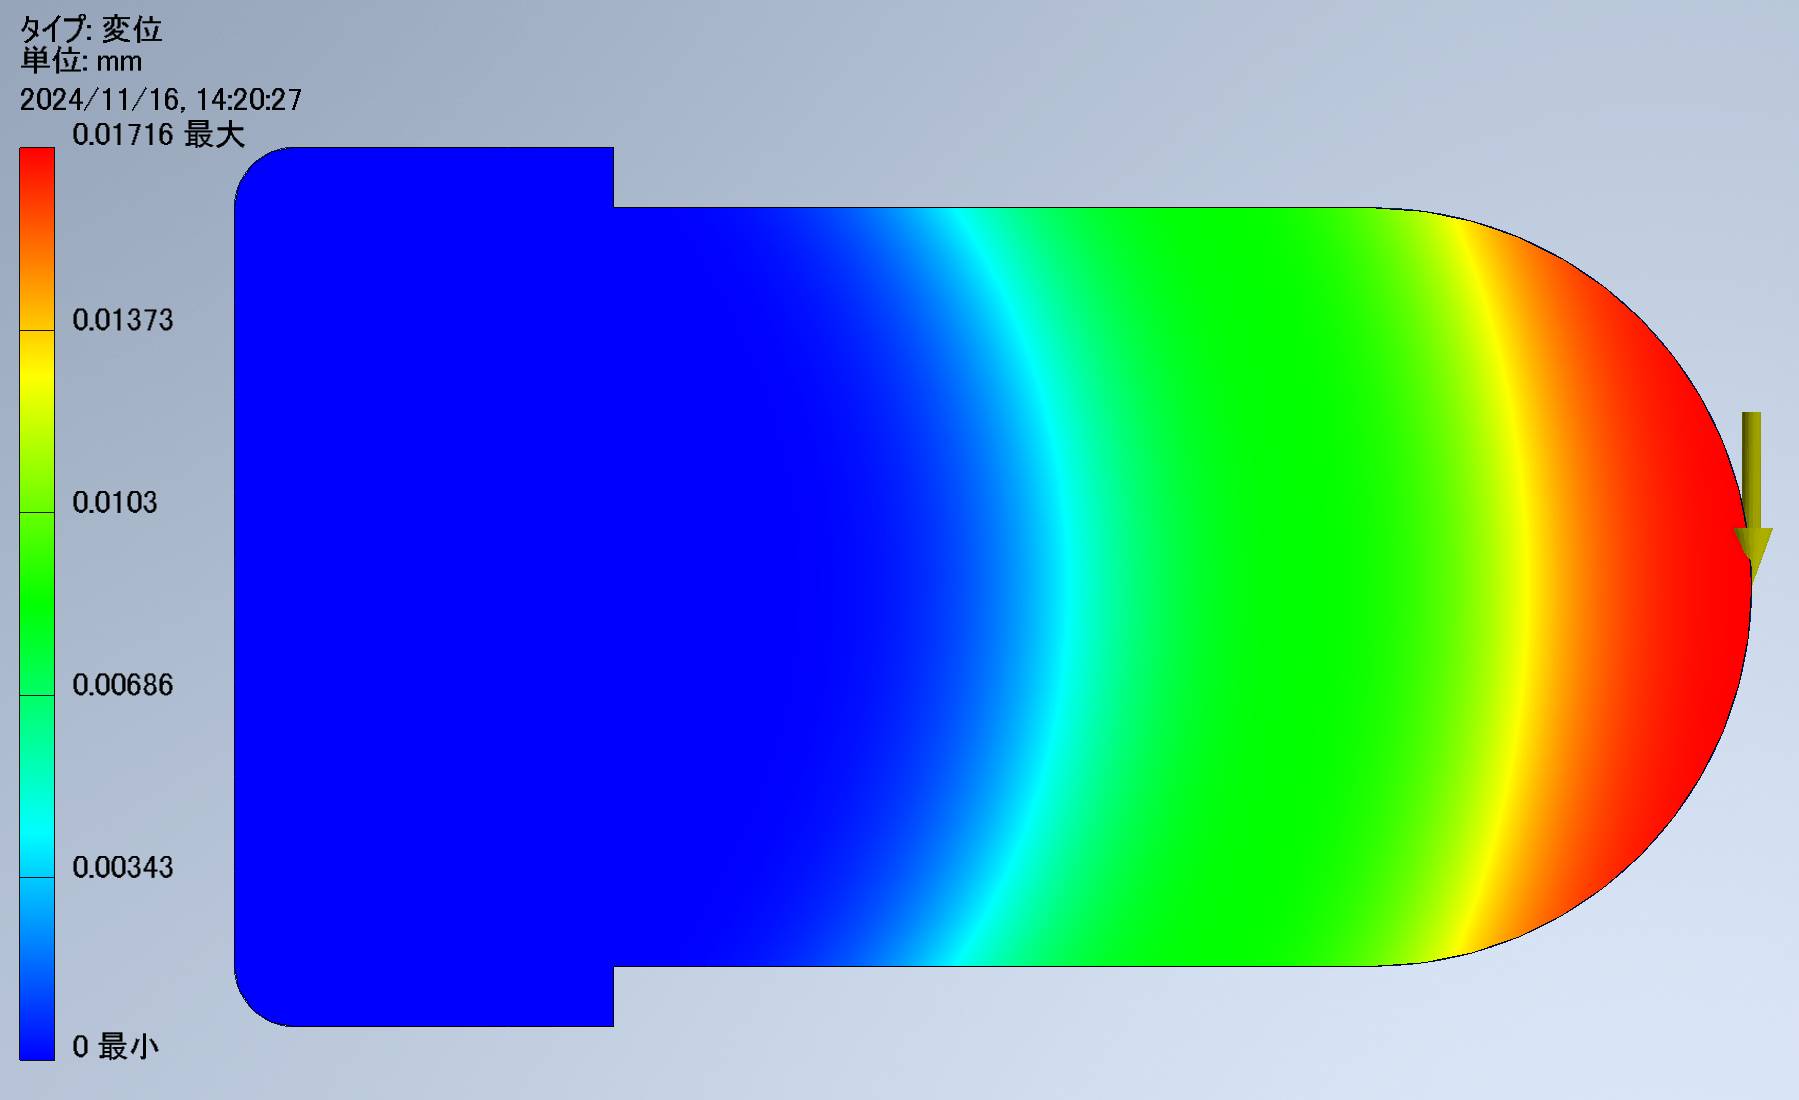
\includegraphics[width=0.99\linewidth]{images/4-3_disp.png}
        \caption{$50\times8[mm^3]$}
        \label{img:4-3_disp}
      \end{minipage}
      \begin{minipage}{.25\textwidth}
        \centering
        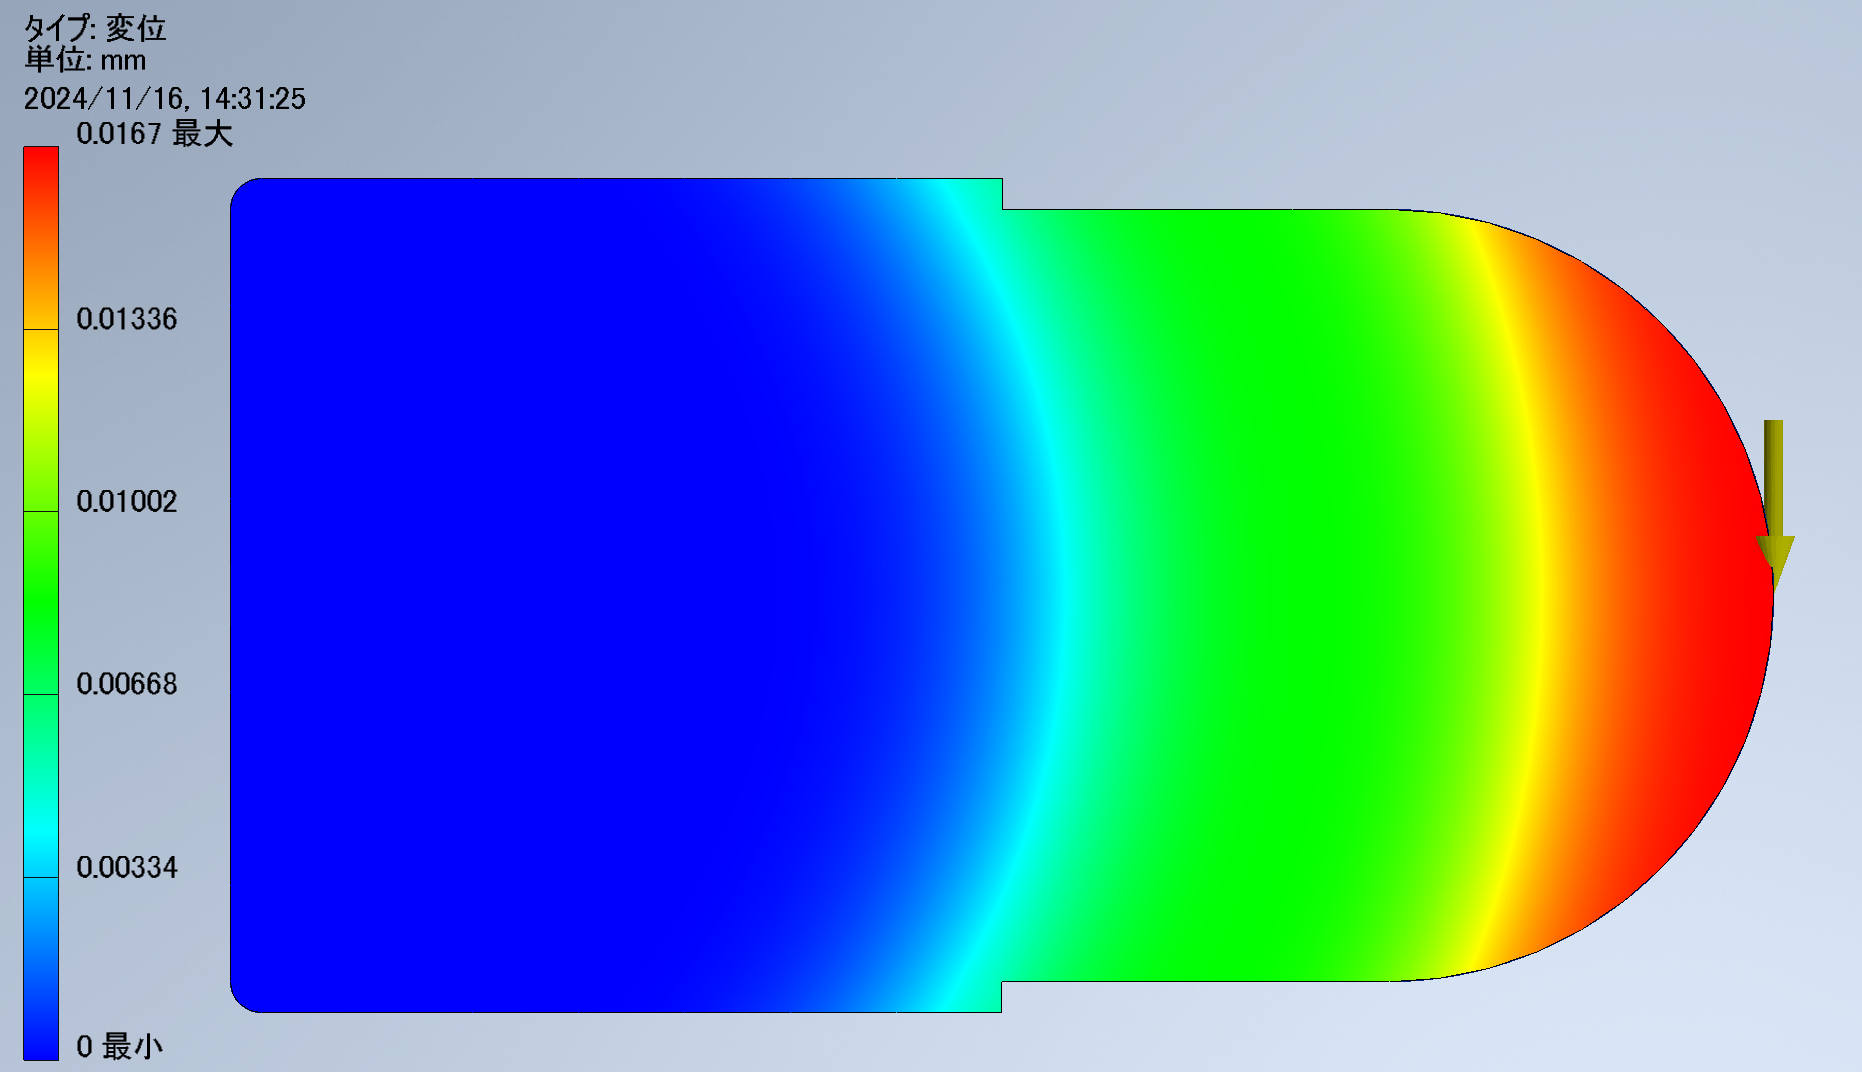
\includegraphics[width=0.99\linewidth]{images/4-6_disp.png}
        \caption{$100\times4[mm^3]$}
        \label{img:4-7_disp}
      \end{minipage}
      \begin{minipage}{.25\textwidth}
        \centering
        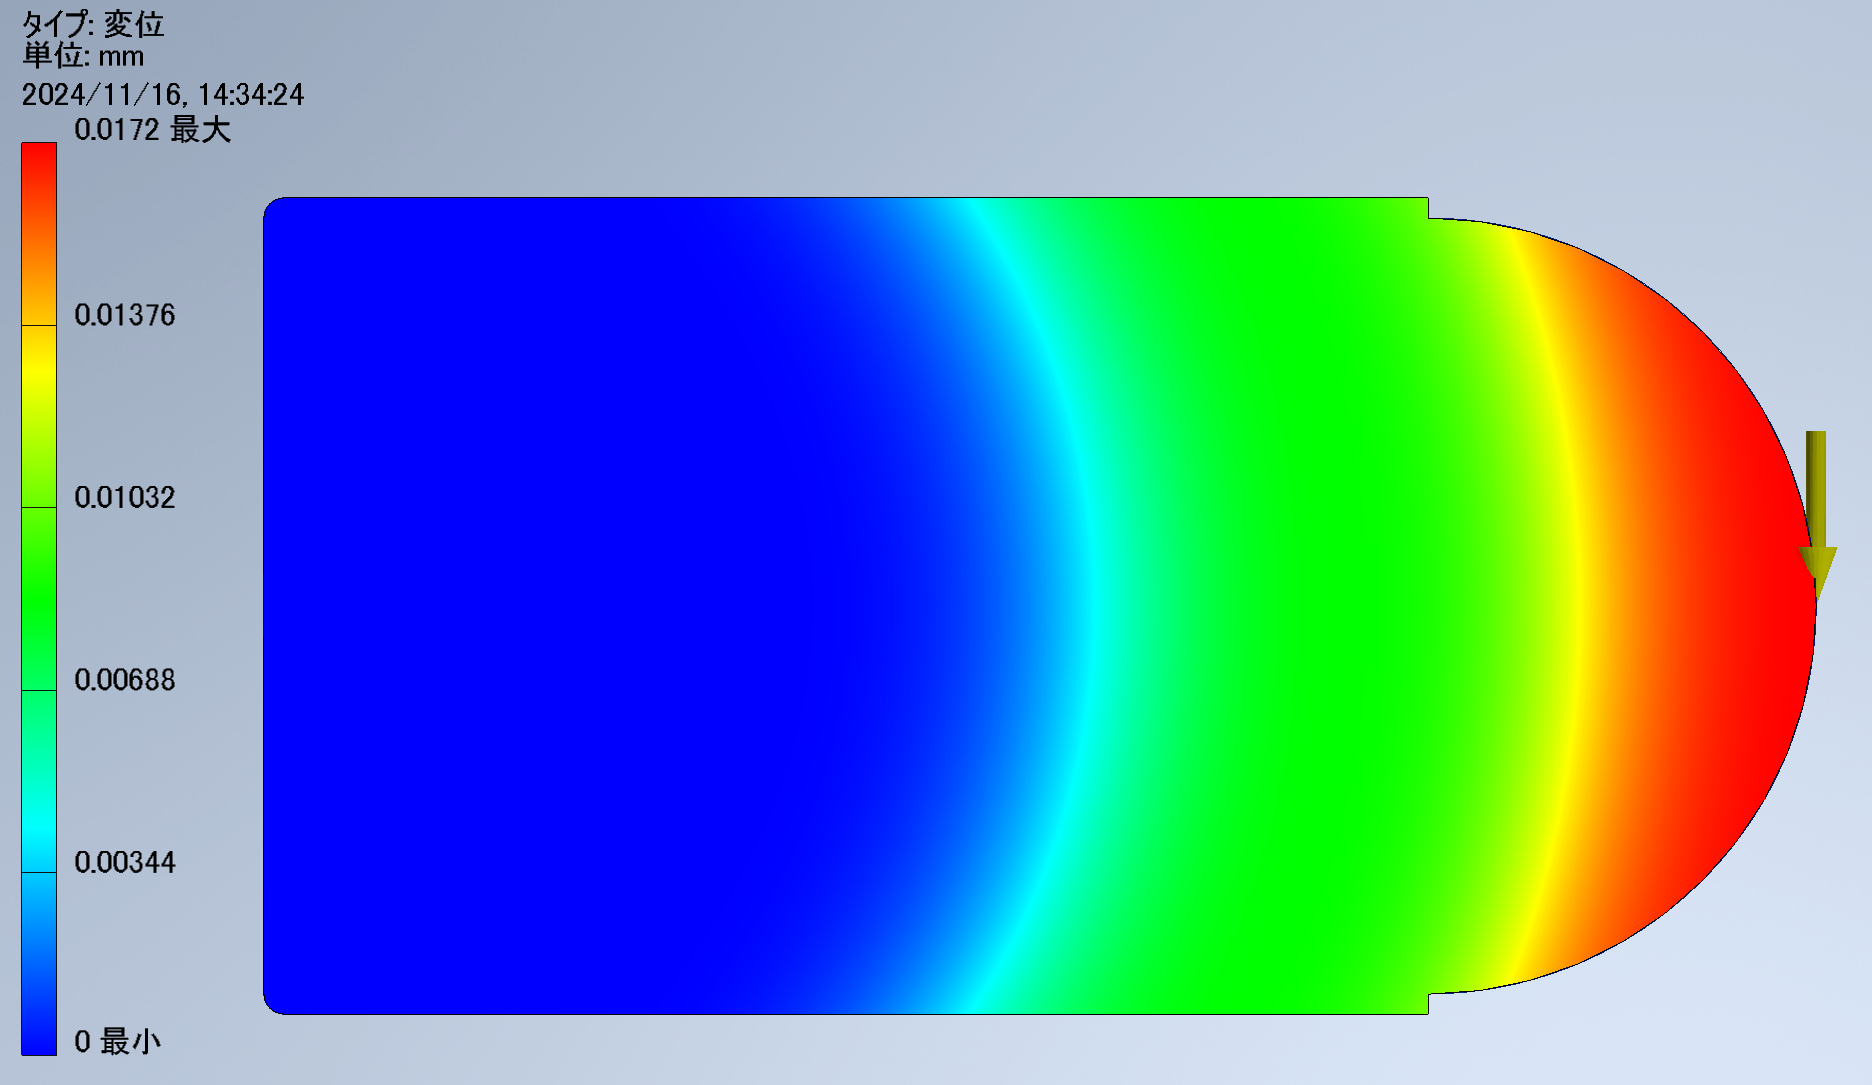
\includegraphics[width=0.99\linewidth]{images/4-7_disp.png}
        \caption{$120\times3.3[mm^3]$}
        \label{img:4-7_disp}
      \end{minipage}
      \begin{minipage}{.25\textwidth}
        \centering
        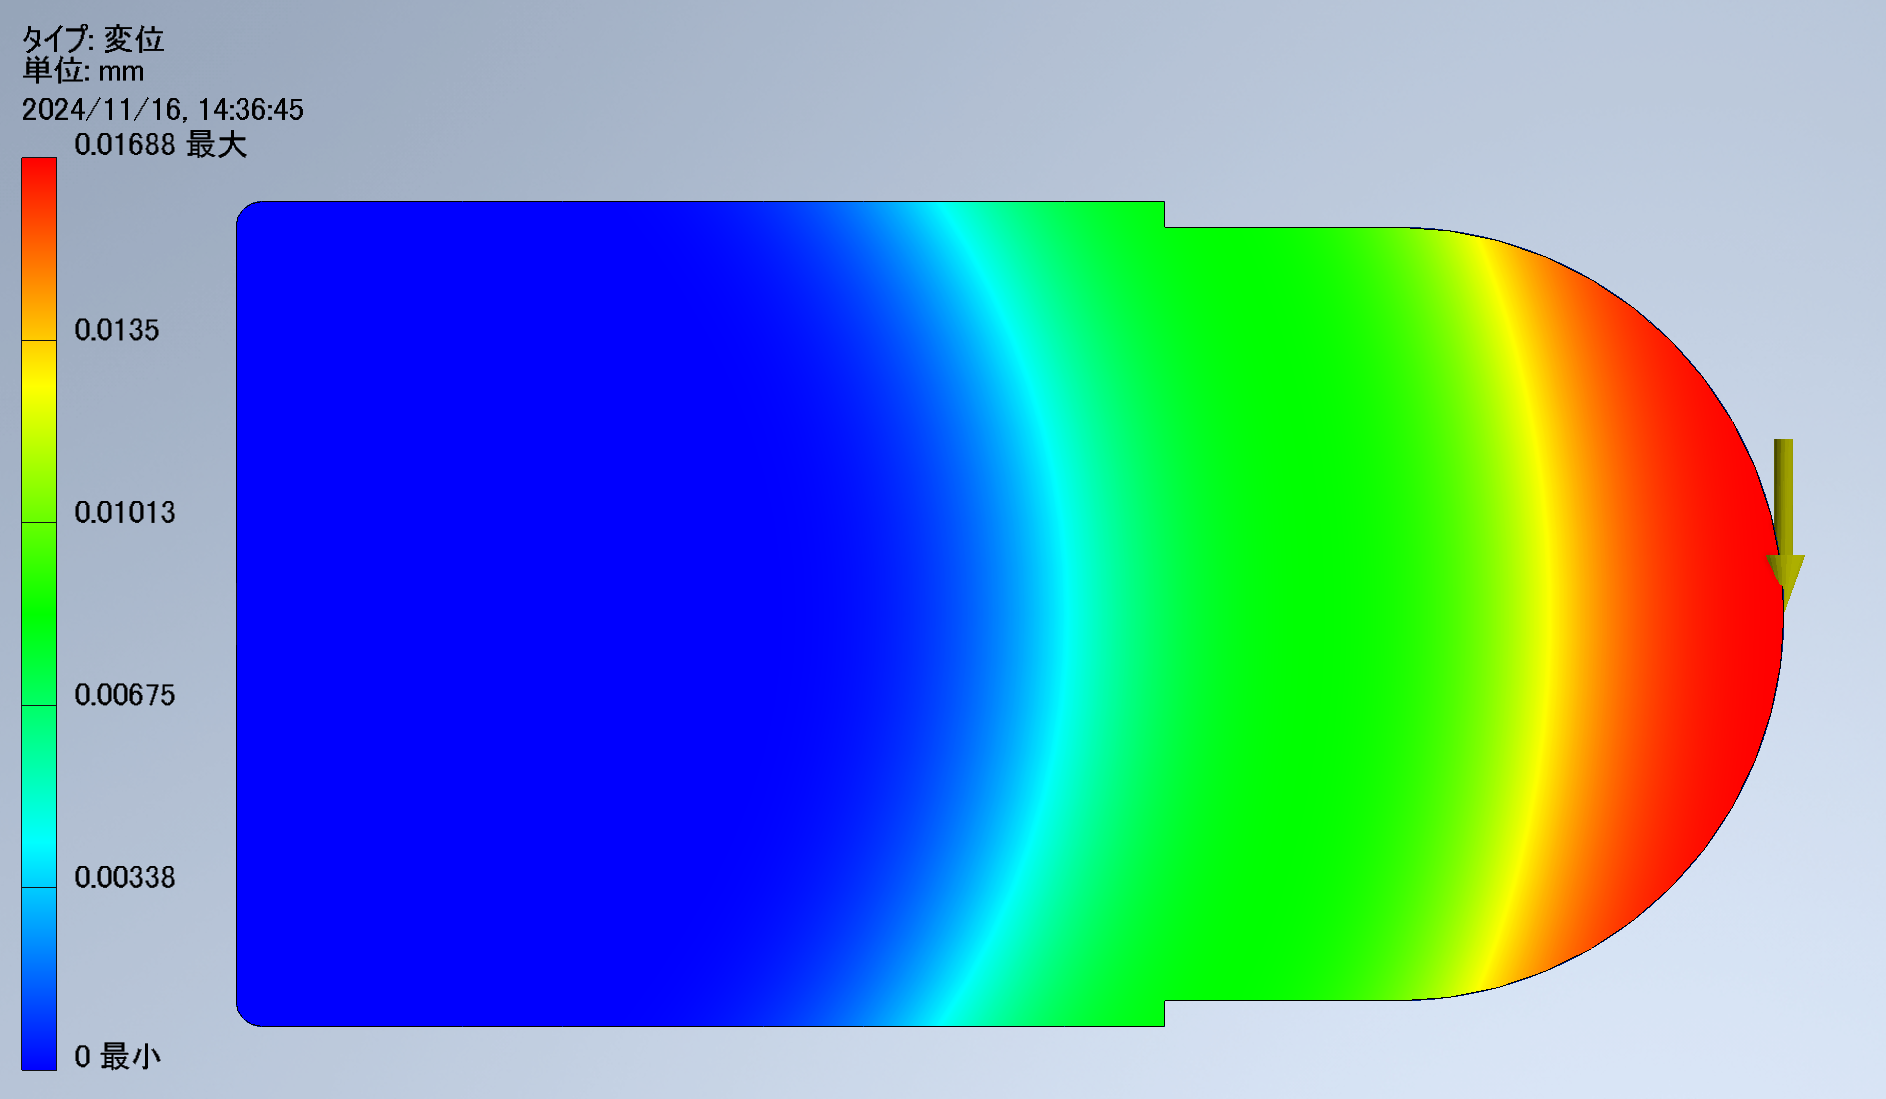
\includegraphics[width=0.99\linewidth]{images/4-8_disp.png}
        \caption{$150\times2.6[mm^3]$}
        \label{img:4-8_disp}
      \end{minipage}
    \end{tabular}
  \end{figure}

  図\ref{img:4-3_voms} - \ref{img:4-8_voms}はそれぞれの応力,
  図\ref{img:4-3_disp} - \ref{img:4-8_disp}はそれぞれの変位.
  以上より変位が最小な$100 \times 4[mm^3]$のパーツで補強した梁を,次の実験で使用する.
